%===================================================================================================
% 実験
%===================================================================================================
\chapter{実験}
%---------------------------------------------------------------------------------------------------
\section{実験内容}
生活空間の物品として,3種類のお菓子,2種類のペットボトル,3種類の醤油入れを想定し,図{\ref{fig:experiment_1_setting}}のように配置した.これらの物品は,三人称センサにより計測され,空間内の物品位置情報がTMSデータベースに管理されているものとする.
実験として,図中の位置からいずれかの物品の方向を向き,その物品名を音声指示として発声した.推定された対象物品は,実環境を模した仮想空間上で図{\ref{fig:arrow}}のように明示される.
%
\begin{figure}[htbp]
  \begin{center}
   \includegraphics[width=130mm]{figure/experiment_1_setting.eps}
   \caption{実験環境}
   \label{fig:experiment_1_setting}
  \end{center}
\end{figure}
%
\begin{figure}[htbp]
\begin{tabular}{cc}
%
  \begin{minipage}{0.3\textwidth}
    \begin{center}
      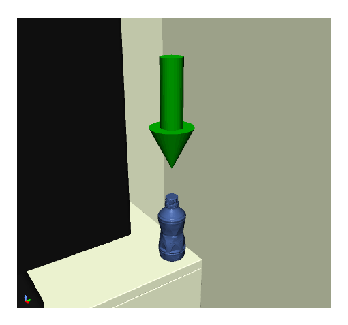
\includegraphics[width=50mm]{figure/arrow.eps}
      \caption{仮想空間上の明示}
      \label{fig:arrow}
    \end{center}
  \end{minipage}
%
  \begin{minipage}{0.7\textwidth}
    \begin{center}
    \makeatletter
    \def\@captype{table}
    \makeatother
    \caption{IDテーブル}
    \label{tb:id_table}
      \begin{tabular}{ccl} \bhline{1.2pt}
        音声指示 & ID & 物品名 \\ \hline
        \multirow{3}{*}{お菓子,ポテトチップス} & 7001 & chipstar\_red \\
        & 7002 & chipstar\_orange \\
        & 7003 & chipstar\_green \\ \hline
        \multirow{2}{*}{ペットボトル,お茶} & 7004 & greentea\_bottle \\
        & 7005 & soukentea\_bottle \\ \hline
        \multirow{3}{*}{醤油} & 7009 & soysauce\_bottle\_black \\
        & 7010 & soysauce\_bottle\_blue \\
        & 7011 & soysauce\_bottle\_white \\ \bhline{1.2pt}
      \end{tabular}
    \end{center}
  \end{minipage}
%
\end{tabular}
\end{figure}

音声内容と候補物品IDの対応を表すテーブルを表{\ref{tb:id_table}}に示す.
表中のIDは,図{\ref{fig:experiment_1_setting}}の物品に添えた数字に対応する.

実験手順は次の通りである.
\begin{enumerate}
\item{ID:7002のお菓子を見ながら,「ポテトチップス」と物品指示}
\item{ID:7005のペットボトルを見ながら,「ペットボトル」と物品指示}
\item{ID:7011の醤油入れを見ながら,「醤油」と物品指示}
\end{enumerate}


%---------------------------------------------------------------------------------------------------
\section{実験結果}
「ポテトチップス」,「ペットボトル」,「醤油」と物品指示を与えた場合の実験結果をそれぞれ図{\ref{fig:experiment_1_result_1}},図{\ref{fig:experiment_1_result_2}},図{\ref{fig:experiment_1_result_3}}に示す.
各図は,左半分に実環境の様子を示し,右半分に仮想空間の様子を示す.
いずれの物品指示においても,所望の物品が推定され,仮想空間に反映された.
これらは,ユーザのジェスチャや,より詳細な追加音声指示などを要求すること無く,視野方向のみを補完情報として正確な指示理解を実現している.
従って,ユーザの視野方向が曖昧な音声指示の理解に有用であることが示された.
%
\begin{figure}[htbp]
\begin{tabular}{cc}
%
  \begin{minipage}{0.5\textwidth}
    \begin{center}
      \includegraphics[width=75mm]{figure/experiment_1_result_1.eps}
    \end{center}
  \end{minipage}
%
  \begin{minipage}{0.5\textwidth}
    \begin{center}
      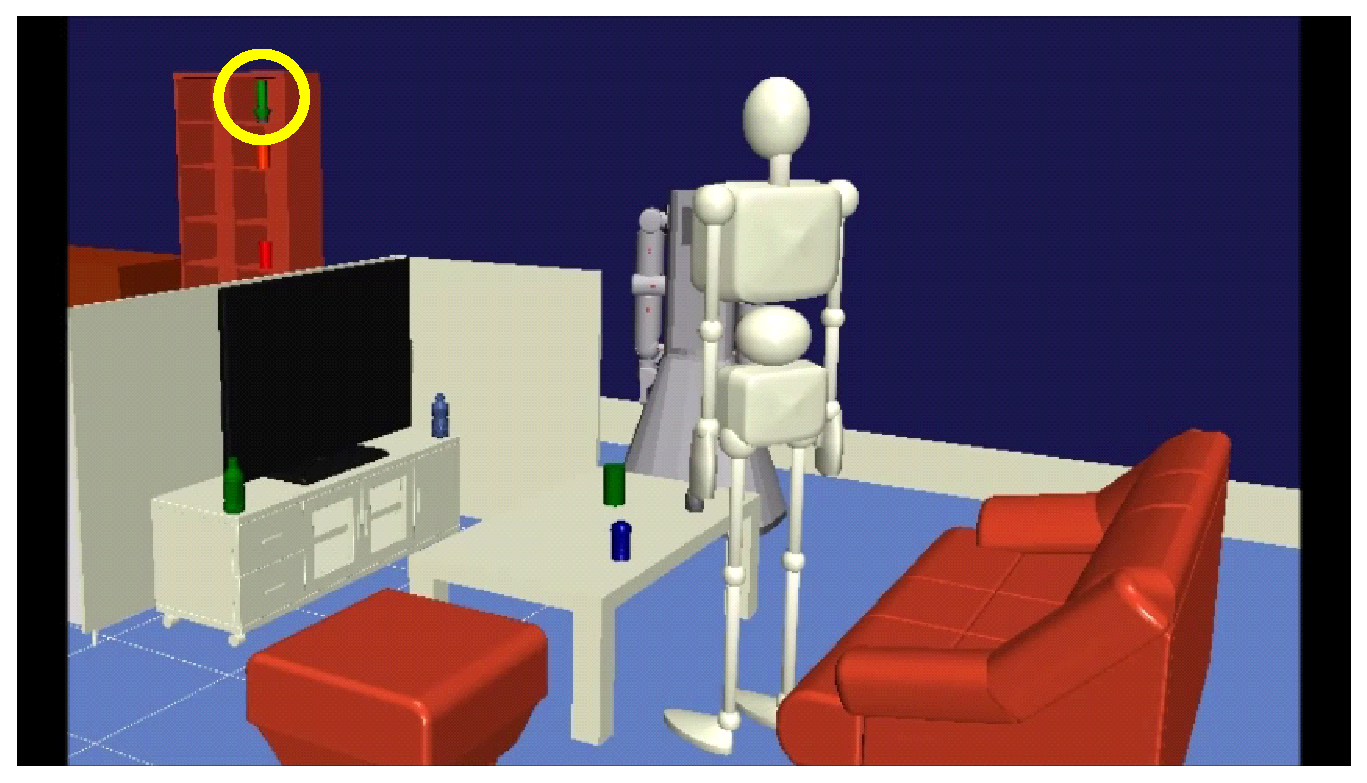
\includegraphics[width=75mm]{figure/experiment_1_result_1_s.eps}
    \end{center}
  \end{minipage}
%
\end{tabular}
\caption{「ポテトチップス」と音声指示を与えた場合}
\label{fig:experiment_1_result_1}
\end{figure}
%
\begin{figure}[htbp]
\begin{tabular}{cc}
%
  \begin{minipage}{0.5\textwidth}
    \begin{center}
      \includegraphics[width=75mm]{figure/experiment_1_result_2.eps}
    \end{center}
  \end{minipage}
%
  \begin{minipage}{0.5\textwidth}
    \begin{center}
      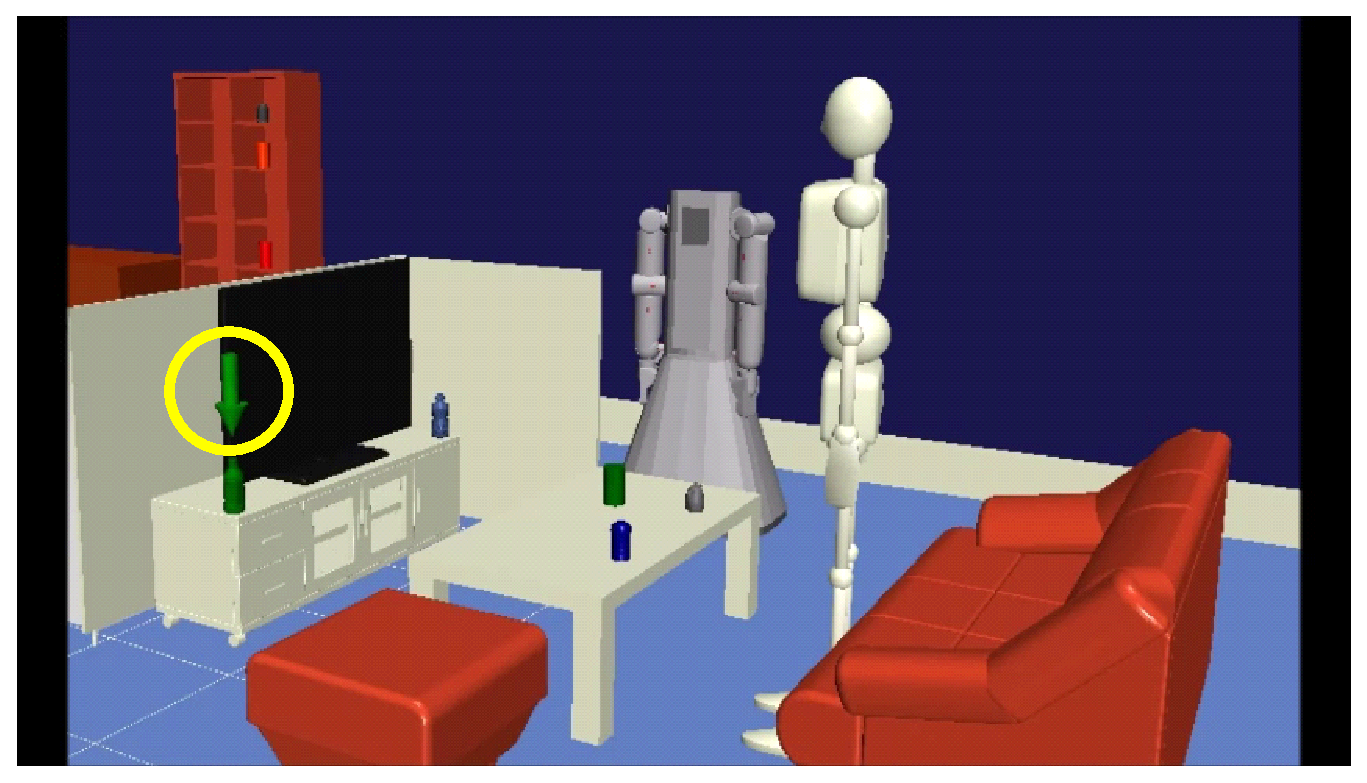
\includegraphics[width=75mm]{figure/experiment_1_result_2_s.eps}
    \end{center}
  \end{minipage}
%
\end{tabular}
\caption{「ペットボトル」と音声指示を与えた場合}
\label{fig:experiment_1_result_2}
\end{figure}
%
\begin{figure}[htbp]
\begin{tabular}{cc}
%
  \begin{minipage}{0.5\textwidth}
    \begin{center}
      \includegraphics[width=75mm]{figure/experiment_1_result_3.eps}
    \end{center}
  \end{minipage}
%
  \begin{minipage}{0.5\textwidth}
    \begin{center}
      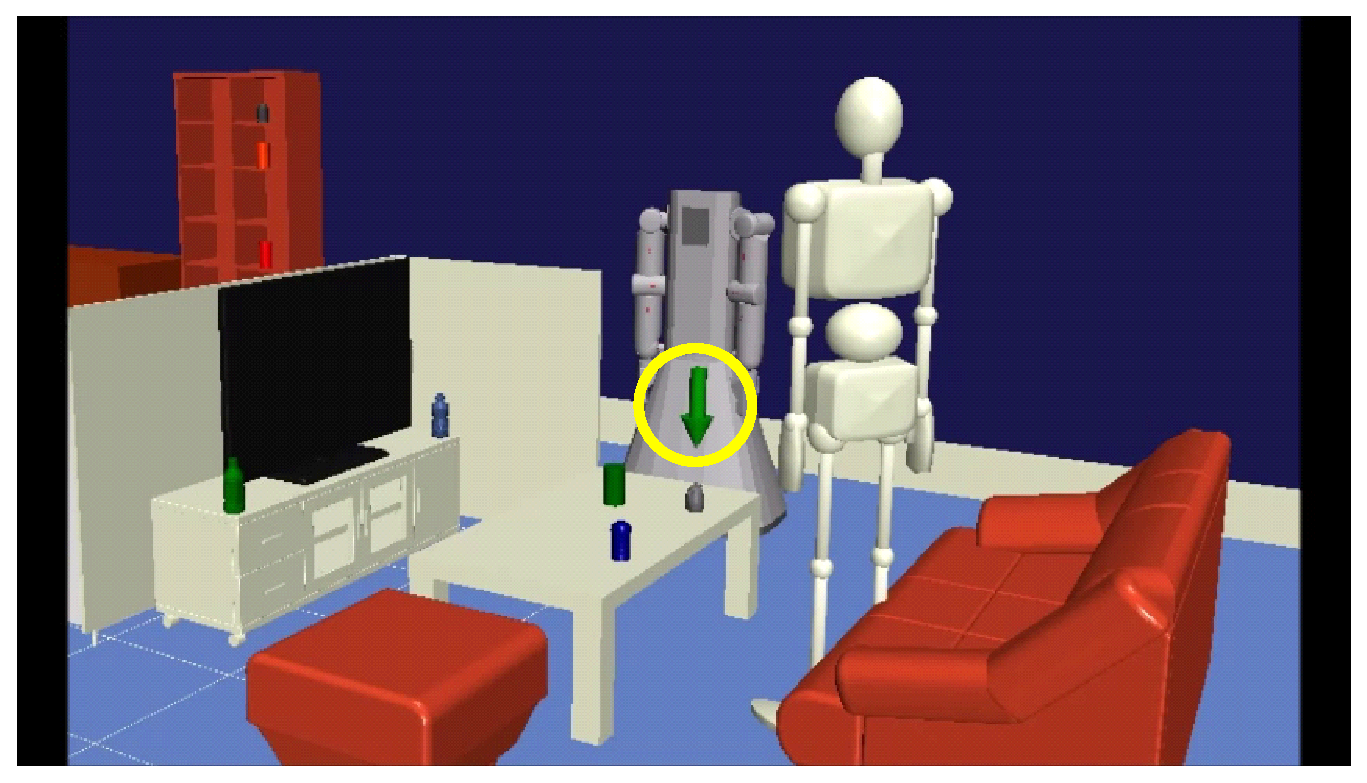
\includegraphics[width=75mm]{figure/experiment_1_result_3_s.eps}
    \end{center}
  \end{minipage}
%
\end{tabular}
\caption{「醤油」と音声指示を与えた場合}
\label{fig:experiment_1_result_3}
\end{figure}